\begin{frame}[t]{Graph Convolutional Network}
    \begin{block}{GCN Setup}
        \begin{itemize}
            \item an input feature matrix $N\times F^0$ feature matrix, $X$, where $N$ is the number of nodes and $F^0$ is the number of input features for each node
            \item an $N\times N$ matrix representation of the graph structure such as the adjacency matrix $A$ of $G$
        \end{itemize}
    \end{block}

    $$ H^i = f(H^{i-1}, A) $$
    $$ = \sigma(AH^{i-1}W)$$

    \begin{block}{Simplification}
        $$ H = AX $$
    \end{block}
\end{frame}

\begin{frame}[t]{Graph Convolutional Network}
    \begin{columns}[onlytextwidth]
        
        \column{.4\textwidth}
        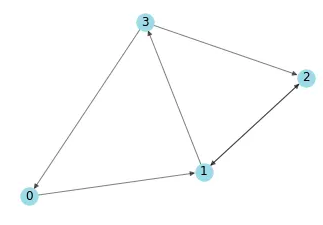
\includegraphics[scale=.38]{images/GCNExampleNet.png}
                                               \column{.6\textwidth}
                                               \begin{math}
                                                    A =
                                                        \begin{bmatrix}
                                                            0 & 1 & 0 & 0\\
                                                            0 & 0 & 1 & 1\\
                                                            0 & 1 & 0 & 0\\
                                                            1 & 0 & 1 & 0
                                                        \end{bmatrix}
                                                    X = \begin{bmatrix}
                                                            0 &  0\\
                                                            1 & -1\\
                                                            2 & -2\\
                                                            3 & -3
                                                        \end{bmatrix}
                                                \end{math}
    \end{columns}

    \begin{block}{Issues}
        \begin{itemize}
            \item Add self loop
            \item Normalize
        \end{itemize}
    \end{block}

    Finally: $f(X, A) = D^{-1} \hat{A} X W$

    \unfootnote{
        \href{https://towardsdatascience.com/how-to-do-deep-learning-on-graphs-with-graph-convolutional-networks-7d2250723780}{How to do Deep Learning on Graphs with Graph Convolutional Networks}
    }
    
\end{frame}

\begin{frame}[t]{GraphSAGE}
    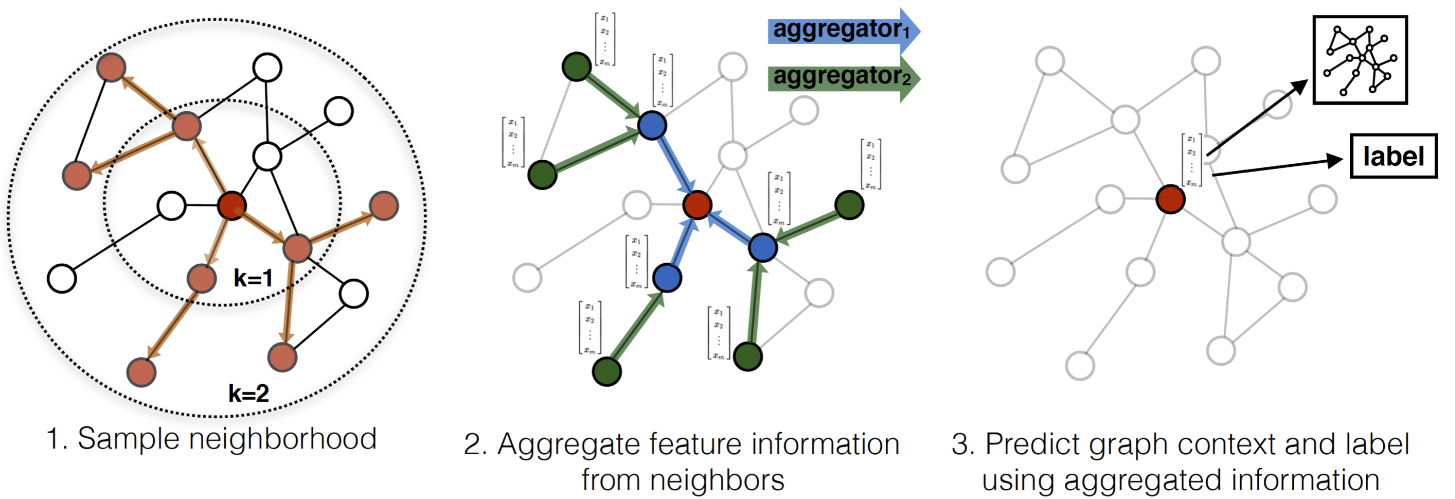
\includegraphics[scale=.2]{GraphSAGE}
    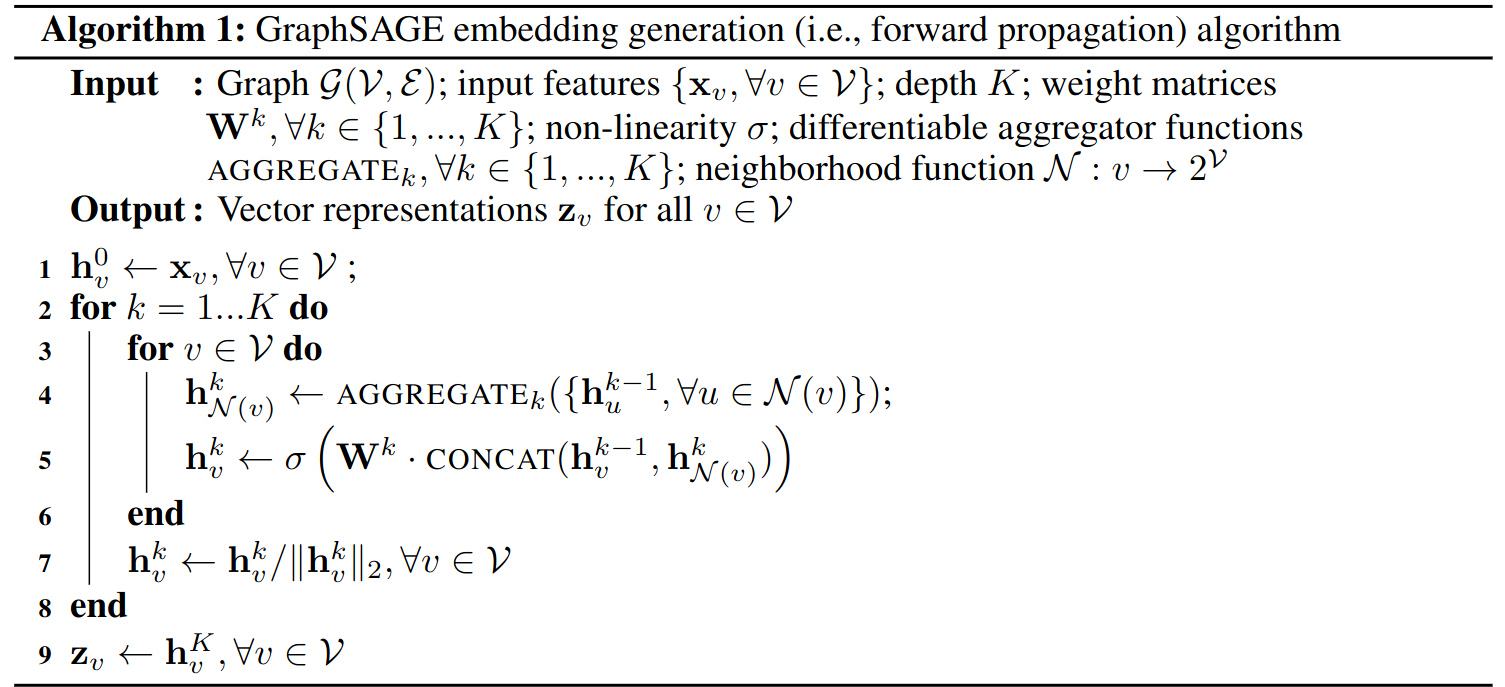
\includegraphics[scale=.18]{GraphSAGEAlgo}
\end{frame}

\begin{frame}[t]{GraphSAGE Loss}
    Encourages nearby nodes to have similar representations, while enforcing
    that the representations of disparate nodes are highly distinct

    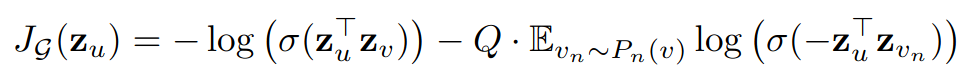
\includegraphics[scale=.27]{GraphSAGELoss}
\end{frame}